\documentclass[hide notes,intlimits]{beamer}

\mode<presentation>
{
  \usetheme{Singapore}
  \usefonttheme{professionalfonts}
  \setbeamertemplate{blocks}[rounded][shadow=true]
  \setbeamercovered{transparent}
}

% load packages
\usepackage[english]{babel}
\usepackage[latin1]{inputenc}
\usepackage[T1]{fontenc}
\usepackage{lmodern}
\usepackage[multidot]{grffile}
\usepackage{verbatim,empheq}
\usepackage{tikz}
\usetikzlibrary{shapes,arrows,shadows}
\usepackage{animate}

\definecolor{dark red}{HTML}{E41A1C}
\definecolor{dark green}{HTML}{4DAF4A}
\definecolor{dark violet}{HTML}{984EA3}
\definecolor{dark blue}{HTML}{084594}
\definecolor{dark orange}{HTML}{FF7F00}
\definecolor{light blue}{HTML}{377EB8}
\definecolor{light red}{HTML}{FB9A99}
\definecolor{light violet}{HTML}{CAB2D6}

\newcommand{\CC}{\mathbb{C}}
\newcommand{\NN}{\mathbb{N}}
\newcommand{\RR}{\mathbb{R}}
\newcommand{\ZZ}{\mathbb{Z}}
\newcommand{\Acal}{\mathcal{A}}
\newcommand{\Bcal}{\mathcal{B}}
\newcommand{\Ccal}{\mathcal{C}}
\newcommand{\Ncal}{\mathcal{N}}
\newcommand{\Kcal}{\mathcal{K}}

\newcommand{\bF}{\mathbf{F}}
\newcommand{\bQ}{\mathbf{Q}}
\newcommand{\bU}{\mathbf{U}}
\newcommand{\bbU}{\bar{\bU}}
\newcommand{\bu}{\mathbf{u}}
\newcommand{\bv}{\mathbf{v}}
\newcommand{\bx}{\mathbf{x}}

\newcommand{\Div}{\nabla\cdot}
\newcommand{\eps}{\epsilon}
\newcommand{\grad}{\nabla}
\newcommand{\lap}{\triangle}
\DeclareMathOperator{\trace}{tr}
\renewcommand{\bar}{\overline}

\newcommand{\ddx}[1]{\frac{\partial #1}{\partial x}}
\newcommand{\ddy}[1]{\frac{\partial #1}{\partial y}}
\newcommand{\pp}[2]{\frac{\partial #1}{\partial #2}}
\newcommand{\ppt}[1]{\frac{\partial #1}{\partial t}}
\newcommand{\ppT}[1]{\frac{\partial #1}{\partial T}}
\newcommand{\ppx}[1]{\frac{\partial #1}{\partial x}}
\newcommand{\ppy}[1]{\frac{\partial #1}{\partial y}}
\newcommand{\ppz}[1]{\frac{\partial #1}{\partial z}}
\newcommand{\ppxx}[1]{\frac{\partial^2 #1}{\partial x^2}}
\newcommand{\ppzz}[1]{\frac{\partial^2 #1}{\partial z^2}}

\newcommand{\Tnorm}[1]{\left|\!\left|\!\left|#1\right|\!\right|\!\right|}
\newcommand{\rhow}{\rho_{\text{w}}}
\newcommand{\Wq}{W^{1,q}(\Omega)}
\newcommand{\half}{\frac12}


\renewcommand{\L}{\emph{Left}}
\newcommand{\R}{\emph{Right}}


\newenvironment{transbox}[1][]{%
\begin{tikzpicture}
\node[drop shadow,rounded corners,text width=\textwidth,fill=white, fill opacity=#1,text opacity=1] \bgroup
}{
\egroup;\end{tikzpicture}}


\title[math tools and obstacles in ice sheet models]{Mathematical tools and obstacles \\ in models of ice sheets}

\author[Bueler]{Ed Bueler}

\institute[UAF]{
  \scriptsize Dept of Mathematics and Statistics and Geophysical Institute \\

  University of Alaska Fairbanks \\
  
  \tiny $^{}$ \\
  \tiny supported by NASA grant \# NNX13AM16G
}

\titlegraphic{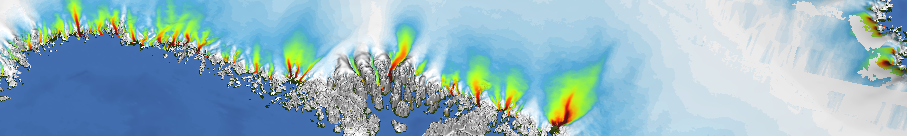
\includegraphics[width=\textwidth]{andycoast.png}}

\setbeamerfont{date}{size=\scriptsize}
\date{}

\AtBeginSection[]
{
  \begin{frame}<beamer>
    \frametitle{Outline}
    %\tableofcontents[currentsection,hideallsubsections]
    \tableofcontents[currentsection]
  \end{frame}
}


\begin{document}

\graphicspath{{../commonfigs/}}

\begin{frame}
\vspace{10mm}
  \titlepage
  \begin{center}
  \tiny Denver University \quad 15 May, 2015
  \end{center}
\end{frame}


\section[intro to ice sheets]{ice sheet flow: an introduction for non-glaciologists}
%\subsection[]{}

\begin{frame}{ice in glaciers is a viscous fluid}
\begin{columns}
\begin{column}{0.65\textwidth}
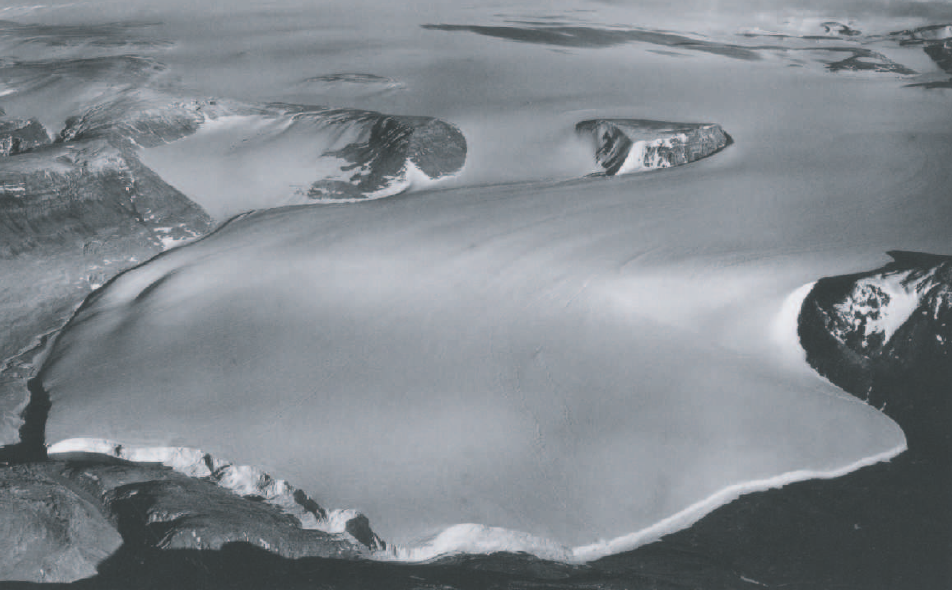
\includegraphics[width=1.0\textwidth]{polaris}
\end{column}
\begin{column}{0.35\textwidth}
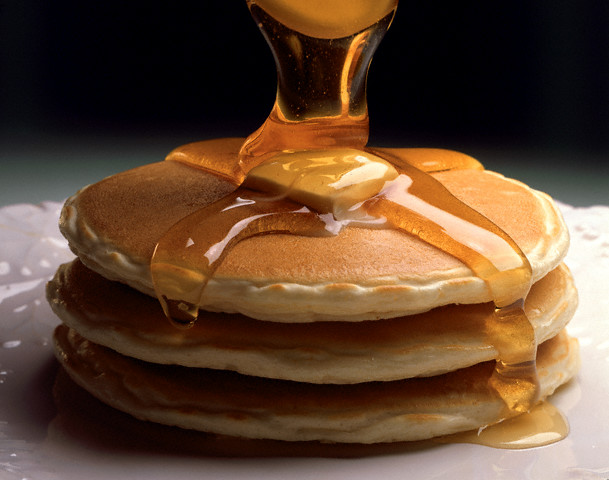
\includegraphics[width=1.0\textwidth]{pancakes}
\end{column}
\end{columns}

\bigskip\bigskip
\begin{itemize}
\item \dots at least: glaciers are viscous flows at larger scales
\item glaciers are free-surface flows (with no surface tension)
\item \emph{usage}: ``ice sheets'' $=$ big, continent-scale glaciers
\end{itemize}
\end{frame}


\begin{frame}{ice in glaciers is a viscous fluid}

\begin{itemize}
\item primary variables: velocity $\mathbf{u}(\bx,t)$ and pressure $p(\bx,t)$
\item also: $\rho$ is density, $\mathbf{g}$ is gravity, $\nu$ is viscosity
\item if the glacier fluid were ``typical'' like the ocean we would model with Navier-Stokes equations:
\begin{align*}
\nabla \cdot \mathbf{u} &= 0 &&\text{\emph{incompressibility}} \\
\rho \left(\mathbf{u}_t + \mathbf{u}\cdot\nabla \mathbf{u}\right) &= -\nabla p + \nu \nabla^2 \mathbf{u} + \rho \mathbf{g} &&\text{\emph{stress balance}}
\end{align*}
\item but ice is not typical!
\item e.g.~not in ice sheet flow models:
  \begin{itemize}
  \item[$\circ$] turbulence
  \item[$\circ$] coriolis force
  \item[$\circ$] convection
  %\item[$\circ$] density-driven flow
  \end{itemize}
\end{itemize}
\end{frame}


\begin{frame}{ice is a slow, shear-thinning viscous fluid}

\begin{itemize}
\item glacier ice is
  \begin{enumerate}
  \item ``slow''\footnote{$Fr\approx 10^{-15}$.  Regarding coriolis: $Fr/Ro \approx 10^{-8}$.}:
    $$\rho \left(\mathbf{u}_t + \mathbf{u}\cdot\nabla \mathbf{u}\right) \approx 0 \qquad \iff \qquad \begin{pmatrix} \text{forces of inertia} \\ \text{are negligible} \end{pmatrix}$$
  \item non-Newtonian shear-thinning\footnote{blood is also shear-thinning \\ \hspace{5mm} corn starch in water is shear-thickening}:
    \begin{itemize}
    \item viscosity $\nu$ is not constant
    \item $\nu$ decreases as fluid is sheared
    \end{itemize}
  \end{enumerate}
\end{itemize}
\end{frame}


\begin{frame}{the standard model}

\begin{itemize}
\item slow flows are called ``Stokes flows''
\item notation:
  \begin{itemize}
  \item[$\circ$] $\tau_{ij}$ is deviatoric stress tensor
  \item[$\circ$] $\mathbf{D}u_{ij}$ is strain rate tensor
  \end{itemize}
\smallskip
\item the standard ice flow model is power-law Stokes:
\begin{align*}
\nabla \cdot \mathbf{u} &= 0 &&\text{\emph{incompressibility}} \\
0 &= - \nabla p + \nabla \cdot \tau_{ij} + \rho \mathbf{g} &&\text{\emph{slow stress balance}} \\
\mathbf{D}u_{ij} &= A \left|\tau_{ij}\right|^{n-1} \tau_{ij} &&\text{\emph{Glen flow law}}
\end{align*}
\item $1.8 < n < 4.0$ ?  \quad \alert{when in doubt: $n=3$}
\medskip
\item $A>0$ is ``ice softness''
   \begin{itemize}
   \item $A$ varies strongly with temperature, but I'll ignore that here
   \end{itemize}
\end{itemize}
\end{frame}


\begin{frame}{model design (because ice is a slow fluid)}

\begin{itemize}
\item ice sheet modeling is a bit like atmosphere flow modeling or weather prediction, but \dots
\item in a Stokes flow, the geometry, boundary stress, and viscosity determine velocity field and pressure, so \dots
\item therefore a time-stepping ice sheet model recomputes the velocity field at every time step, without requiring previous velocity\footnote{to be a weatherman you've got to know which way the wind blows \dots but not to be a glaciologist}
\end{itemize}
\end{frame}


\begin{frame}{sheets versus streams versus shelves}

\begin{columns}
\begin{column}{0.35\textwidth}
\small
\begin{itemize}
\small
\item non-sliding portions of ice sheets flow by shear deformation
\item ice streams slide too
\item ``ice shelves'' are floating thick ice \dots all sliding
\item ice shelves flow by extension not shear
\item but: sliding ignored for today
\end{itemize}
\end{column}

\begin{column}{0.65\textwidth}
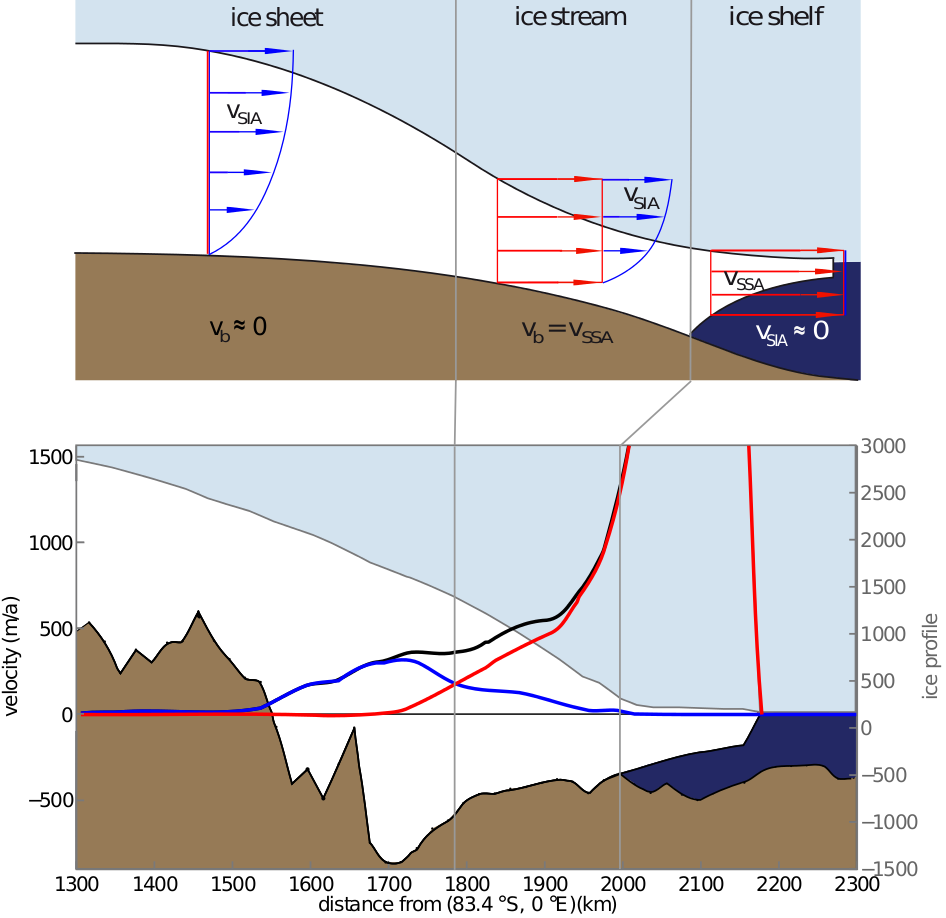
\includegraphics[width=\textwidth]{siassacartoon-lambert}

\begin{center}
\vspace{-0.18in}
\tiny [Lambert glacier and Amery ice shelf, Antarctic]
\end{center}
\end{column}
\end{columns}
\end{frame}


\begin{frame}{ice sheets are shallow}

\begin{itemize}
\item cross-section of Greenland ice sheet at $71^\circ$ N
\small
  \begin{itemize}
  \item[$\circ$] {\color{dark green}{green}} and {\color{dark blue}{blue}}: usual vertically-exaggerated version
  \end{itemize}
  \begin{center}
    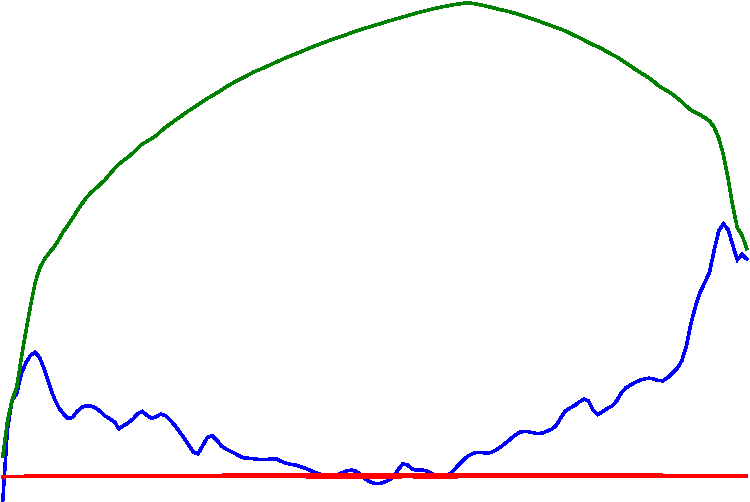
\includegraphics[width=0.5\textwidth]{newgreentrans}
  \end{center}
\normalsize
\item in {\color{dark red}{red}}: a view without this vertical exaggeration
\item \emph{thus}: 
  \begin{itemize}
  \item[$\circ$] most simulations use shallow limits of Stokes
  \item[$\circ$] \scriptsize technical: high aspect-ratio elements bad in non-shallow solvers
  \end{itemize}
\end{itemize}
\end{frame}


\begin{frame}
  \frametitle{first big picture: ice sheets store past climates}
Greenland layers movie from NASA, January 2015
\end{frame}


\begin{frame}
  \frametitle{second big picture: ice sheets affect sea level}
\medskip
\small
\begin{itemize}
\item \emph{mass and energy inputs}: (1) snow adds, (2) sun heats, (3) ocean heats, (4) earth heats
\item \emph{mass outputs}: (1) surface meltwater, (2) basal meltwater, (3) ice discharge
\end{itemize}
\begin{center}
  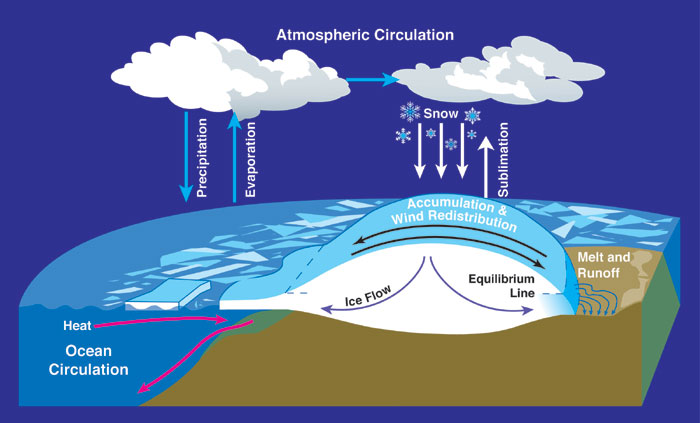
\includegraphics[width=0.75\textwidth]{mass-bal-atmos}
  %\tiny (figure from IceSAT brochure)
\end{center}
\end{frame}


\begin{frame}{summary so far}
\begin{itemize}
\item ice sheets have five outstanding properties \emph{as viscous flows}:
  \begin{enumerate}
  \item \alert{free surface}
  \item \alert{slow}
  \item \alert{shear-thinning}
  \item \alert{shallow}
  \item \alert{sliding (``contact slip'')}
  \end{enumerate}
\end{itemize}
\end{frame}


\section[shallow ice well-posed?]{is the shallow ice problem well-posed and approximate-able?}


\begin{frame}
  \frametitle{shallow ice approximation (SIA)}

\begin{itemize}
\item SIA = lubrication approximation of Stokes model
\item good approximation when:
  \begin{itemize}
  \item[$\circ$] sliding is small or zero
  \item[$\circ$] bedrock slope is modest
  \end{itemize}
\item derive SIA equations by scaling Stokes:
  \begin{itemize}
  \item[$\circ$] $[h]$ is a typical thickness scale
  \item[$\circ$] $[x]$ is a typical width scale
  \item[$\circ$] small parameter is $\eps = [h] / [x]$
  \end{itemize}
\end{itemize}
\end{frame}


\begin{frame}
  \frametitle{SIA: velocity}
 
\begin{itemize}
\item $b(x,y)$ is bedrock elevation (data)
\item $s(x,y,t)$ is ice surface elevation (unknown)
\item let $p=n+1>2$
\item assume: no sliding and isothermal
\item horizontal ice velocity is given by: 
  $${\bf U}  =  - \frac{p}{p+1} \Gamma \left[ (s-b)^p - (s - z)^p  \right] 
|\nabla s |^{p-2} \nabla s$$
where $\Gamma > 0$ combines gravity, ice density, ice softness
\end{itemize}
\end{frame}


\begin{frame}
  \frametitle{SIA plus mass conservation in steady state}

\begin{itemize}
\item $a(x,y)$ is snowfall or melt rate (``surface mass balance''; data)
\item mass conservation in steady state: 
  $$\Div \left(  \int_b^s {\bf U}\, dz \right)  =  a$$
\item shallow ice approximation + (steady) mass conservation:
  $$- \Div \left(\Gamma (s-b)^{p+1} | \nabla s |^{p-2} \nabla s  \right) =  a$$
  \begin{itemize}
  \vspace{-0.2in}
  \item[$\circ$] this is the SIA equation
  \item[$\circ$] $p$-Laplace-ish \dots but coefficient $(s-b)^{p+1} \to 0$ at margins
  \end{itemize}
\item equation above is simplest model for turning data of problem ($b$ and $a$) into ice sheet geometry and velocity ($s$ and $U$)
\end{itemize}
\end{frame}


\begin{frame}{movie of time-dependent SIA}

\begin{columns}
\begin{column}{0.4\textwidth}
\small
\begin{itemize}
\item time-dependent SIA
  $$\frac{\partial s}{\partial t} = a - \Div \left(  \int_b^s {\bf U}\, dz \right)$$
\end{itemize}
\end{column}

\begin{column}{0.65\textwidth}
\vspace{-0.25in}

\begin{center}
\animategraphics[autoplay,loop,height=5.2cm]{4}{../commonfigs/animhalfar/halfar}{0}{26}

\bigskip
\tiny
frames from $t=4$ months to $t = 10^6$ years,

equal spaced in \emph{exponential} time
\end{center}
\end{column}
\end{columns}


\begin{itemize}
\scriptsize
\item the Halfar (1983) similarity solution:
  \begin{itemize}
  \scriptsize
  \item[$\circ$] an exact $b=0,a=0$ solution with $t\to 0^+$ limit a delta function
  \item[$\circ$] compare Barenblatt solution of porous medium equation
  \end{itemize}
\end{itemize}
\end{frame}


\begin{frame}
  \frametitle{SIA: an analogy}
\begin{columns}
\begin{column}{0.4\textwidth}
\begin{itemize}
\item ice sheet surface \\ $\sim$ \alert{membrane}
\item bedrock $\sim$ \alert{obstacle}
\end{itemize}
\begin{center}
\vspace{-2mm}
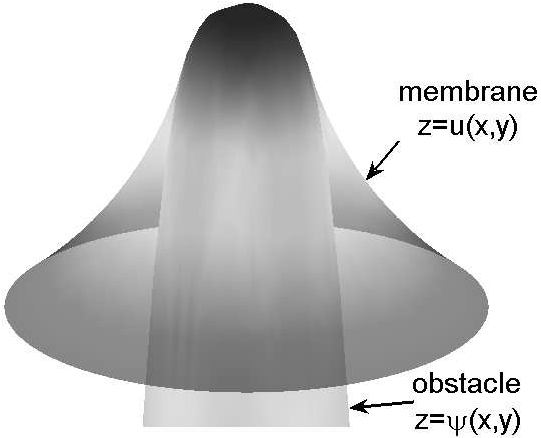
\includegraphics[width=\textwidth]{classicalobs}
\begin{itemize}
\item classical Laplacian obstacle problem:
   $$\lap u = 0 \quad \& \quad u\ge \psi$$
\end{itemize}
\end{center}
\end{column}
\begin{column}{0.55\textwidth}
\begin{center}
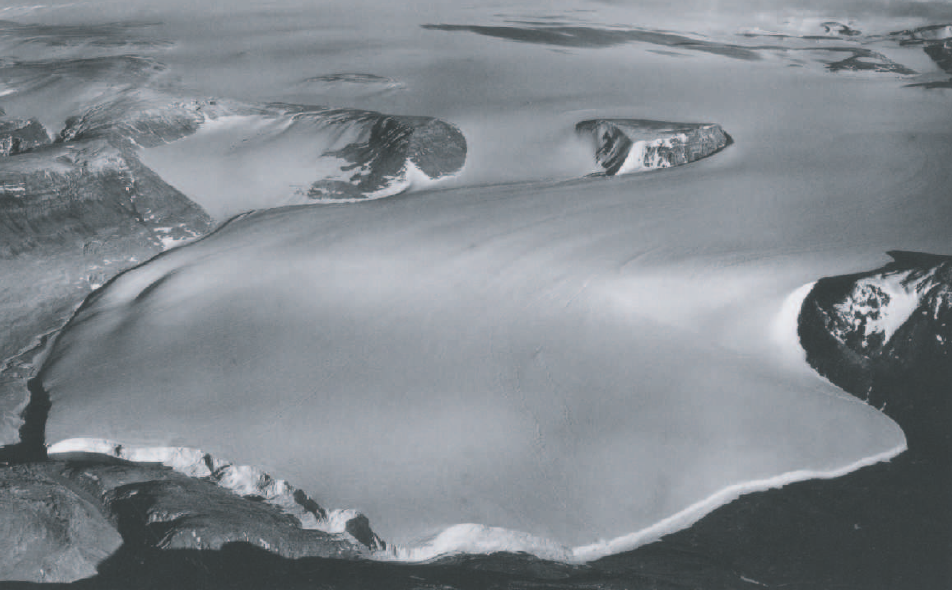
\includegraphics[width=0.95\textwidth]{polaris} \\
\vspace{10mm}
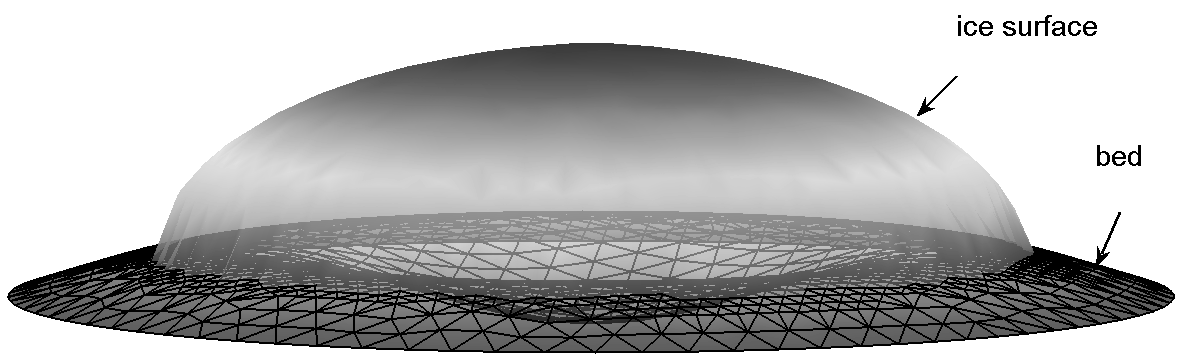
\includegraphics[width=1.05\textwidth]{capnonflatobs}
\end{center}
\end{column}
\end{columns}
\end{frame}


\begin{frame}
  \frametitle{weak formulation = variational inequality} 

\begin{itemize}
\item $H=s-b$ is ice thickness
\item SIA equations apply only where $s>b \iff H > 0$
\item define convex admissible set
  $$\Kcal := \{\eta : \eta^{2p/(p-1)} \in W^{1,p}_0 (\Omega) \,\text{and}\, \eta \ge 0\}$$
over larger domain $\Omega \subset \RR^2$
\end{itemize}

\begin{block}{definition} 
$H \in \Kcal$ solves the \emph{steady shallow ice sheet problem} if
  $$\int_{\Omega}  \Gamma H^{p+1} |\grad s|^{p-2} \grad s \cdot \grad(\eta - H)  
\ge \int_{\Omega} a (\eta - H)$$
for all $\eta \in \Kcal$
\end{block}
\end{frame}


\begin{frame}
  \frametitle{on well-posedness (Jouvet-Bueler 2012)} 

\begin{block}{theorem.}
if $b=0$ then variational inequality is equivalent to minimizing
  $$J[\eta] = \int_{\Omega} \frac{\Gamma}{p} |\grad u|^p - a u$$
over $u^{(p-1)/(2p)} = \eta \in \Kcal$, and this problem is well-posed (existence, uniqueness, stability w.r.t.~data $a$)
\end{block}

\begin{block}{theorem.}
in general case ($b\ne 0$) there exists a solution
\end{block}

\begin{proof}[proof]
fixed-point theorem, of course
\end{proof}
\end{frame}


\begin{frame}
  \frametitle{another weak form} 

FIXME: v.i. $\iff$ n.c.p.
\end{frame}


\begin{frame}
  \frametitle{an interesting quality} 

\begin{itemize}
\item every glaciologist believes this about steady climates:
	$$\text{if } a > 0 \text{ on } R \text{ then } H > 0 \text{ on } R$$
\item that is:
\begin{center}
 if it snows more than it melts then you get a glacier
\end{center}
\end{itemize}

\begin{columns}
\begin{column}{0.6\textwidth}
\begin{itemize}
\small
\item uniformly-elliptic variational inequalities, e.g.~the classical obstacle problem,
\begin{align*}
\int_{\Omega}  \nabla u \cdot \nabla (v - u)  \ge  \int_{\Omega} f (v - u),
\end{align*}
for all $v\ge \psi$, do \emph{not} have the analogous property
\end{itemize}
\end{column}
\begin{column}{0.4\textwidth}
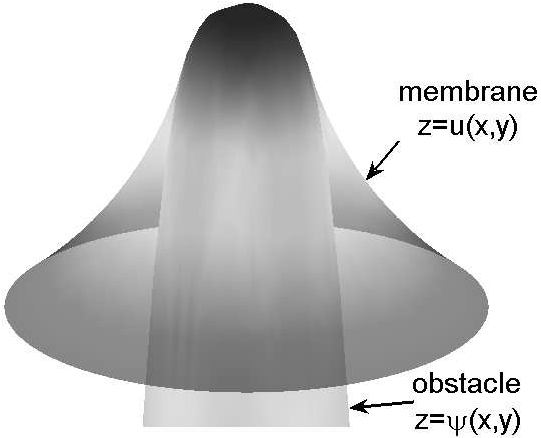
\includegraphics[width=\textwidth]{classicalobs}
\end{column}
\end{columns}
\end{frame}


\begin{frame}
  \frametitle{example: steady Greenland ice sheet}

\begin{columns}
\begin{column}{0.5\textwidth}
\begin{itemize}
\item NCP solved by continuation scheme $+$ Newton iteration from PETSc on 900m grid using 192 processes
\end{itemize}
\end{column}
\begin{column}{0.5\textwidth}
FIXME updated image from siafve
\end{column}
\end{columns}

\end{frame}


\section[conservation w free boundaries?]{can thin-layer free-boundary models be exact-discrete-conserving?}
%\subsection[]{}

\begin{frame}
  \frametitle{FIXME} 

FIXME
\end{frame}


\section*{conclusion}

\begin{frame}
  \frametitle{conclusion}

\begin{itemize}
\item is shallow ice problem
  \begin{itemize}
  \item[$\circ$] well-posed? \qquad \alert{probably}
  \item[$\circ$] approximate-able? \qquad \alert{yes} (but how fast and reliably?)
  \end{itemize}
\item can thin-layer free-boundary problems
  \begin{itemize}
  \item[$\circ$] be solved by implicit time-stepping? \qquad \alert{yes}
  \item[$\circ$] be exactly discrete conserving? \qquad \alert{no}
  \end{itemize}
\end{itemize}
\end{frame}

\end{document}
